\chapter{Algoritmy umělé inteligence}
V této kapitole se seznámíme se dvěma přístupy, které spadají do odvětví umělé inteligence. 
Představíme jejich základní myšlenku. Zmíníme, kde se tyto algoritmy dají použít a v následující kapitole je i využijeme v našem herním prostředí pro trénování inteligentních agentů.

\section{Genetické programování}

\subsection{Základní princip}
Genetické programování je evoluční technika, která vytváří počítačové programy. Cílem genetického programování je vyřešit co nejlépe zadaný problém.
Nespecifikujeme jak je potřeba ho vyřešit, ale víme, co je potřeba vyřešit.
\par
Každý program budeme nazývat jedincem a množině jedinců budeme říkat populace. Algoritmus pak běží iterativně v generacích. 
V každé iteraci se provede výběr nějakých jedinců z populace, ti se pomocí genetických operátorů upraví a nakonec se rozhoduje, kteří z nich přežijí do další generace.
Populaci na začátku iterace nazýváme rodiče a populaci, která bylo nakonci iterace pro další generaci, nazýváme potomky.
Každý program představuje jedno řešení daného problému. Kvalitu tohoto řešení ohodnocujeme takzvanou fitness funkcí. Čím vyšší hodnotu této funkce jedinec získá, tím lépe řeší daný problém.


\subsubsection{Reprezentace}
Program je obvykle reprezentovaný syntaktickým stromem. Stromy ve vnitřních uzlech obsahují funkce (neterminály) a v listech terminály.
Vyhodnocení stromu probíhá od listů ke kořeni a výsledek programu je pak hodnota kořenu.


\subsubsection{Inicializace populace}
Na začátku evoluce potřebujeme inicializovat populaci. Na počátku jsou jedinci vytvořeni náhodně. Obvykle se k vytvoření jedinců používají dvě metody.
První z nich je vytváření jedinců s pevně danou hloubkou stromu, kde v listech jsou vždy už jen terminály. Druhou metodou je stavět strom náhodně z předem daného počtu neterminálů.
Po vyčerpání počtu neterminálů se již opět přidají terminály jako listy. Tato metoda vytváří jedince různých velikostí a tvarů.
Častou praxí je prvotní populaci vytvořit tak, že každá z metod vytvoří polovinu jedinců. 


\subsubsection{Selekce}
V každé iteraci chceme vybrat několik jedinců, nad kterými budeme provádět různé genetické operátory. Snahou je vybírat jedince s vyšší hodnotou fitness funkce.
Asi nejpoužívanější metodou selekce je turnajová selekce. Náhodně se zvolí daný počet jedinců, ti se porovnají mezi sebou na základě jejich hodnoty fitness funkce a nejlepší z nich je pak zvolen do výběru.
Dalším z mnoha metod selekce je ruletová selekce. Zde je pravděpodobnost zvolení jedince do výběru přímo úměrná jeho hodnotě fitness funkce.
Pravděpodobnost výběru i-tého jedince je 
\[p(i) = \frac{f(i)}{\sum_{j=1}^{n} f(j)}. \]
Ruletová selekce má jednoduchou implementaci a zároveň je rychlá na výpočet. 
Jejím problémem je ale předčasná konvergence k lokálnímu optimu.
\par
Genetické operátory mohou občas upravit nejlepšího jedince tak, že se jeho hodnota fitness funkce výrazně zhorší.
Z tohoto důvodu se často používá technika zvaná elitismus, která automaticky do další generace vybere několik nejlepších současných jedinců. 
Tímto způsobem máme zajištěno, že neztratíme nejlepší jedince.

\url{https://www.researchgate.net/publication/259461147_Selection_Methods_for_Genetic_Algorithms}


\subsubsection{Genetické operátory}
Genetické operátory jsou dvojího druhu, křížení a mutace. Myšlenkou křížení je vzít dva jedince, nazývejme je rodiče, a pomocí křížení informací každého z nich vytvořit nového potomka.
V genetickém programování pracujeme s jedinci reprezentovanými stromy, proto křížení jedinců představuje křížení jejich stromů. V každém z rodičů se zvolí jeden uzel. 
Výsledný potomek vypadá jako první rodič, jen na původním místě vybraného uzlu bude nyní podstrom, který je zavěšený pod vybraným uzlem druhého rodiče.
\par
Druhým genetickým operátorem je mutace, ta již nepotřebuje mít dva rodiče, ale úprava se provede nad jedincem samotným.
Mutovat můžeme v jedinci buď jediný bod, nebo celý nějaký podstrom. V případě mutace podstromu se namísto vybraného podstromu vygeneruje zcela nový podstrom. 
Toto v zásadě představuje křížení s novým náhodně vytvořeným jedincem.
\newline
Mutace jediného bodu změní náhodně jediný uzel ve stromě. V případě terminálu se může vybrat libovolný jiný terminál. A v případě vnitřního uzlu může být vybraný libovolný jiný neterminál, který je stejné arity.


\subsubsection{Silná a volná typovanost}
Ve volně typovaném genetickém programování nezadáváme typy funkcí ani terminálů. Jediné co musíme u funkcí určit je jejich arita a na základě toho se generují a mutují jedinci korektně.
Obvykle se nám více bude hodit silně typované genetické programování, zde určujeme u všech funkcí nejen jejich aritu, ale také typ každého z argumentů dané funkce a také typ návratové hodnoty.
Podobně musíme určit i hodnotové typy terminálů. Díky tomu máme zaručeno, že pokud máme například funkci, která vrací typ boolean, tak tato hodnota nebude vynásobena hodnotou typu float. 
Pak jen určíme hodnotové typy celého problému a algoritmus už se postará o to, aby byly typové podmínky dodrženy.
\url{https://deap.readthedocs.io/en/master/tutorials/advanced/gp.html}


\subsection{Využití}
Genetické programování je využitelné ve všech problémech, kde jsme schopní vymyslet způsob jak reprezentovat jedince představujícího řešení problému a fitness funkci, díky které jsme schopni dané řešení ohodnotit.
To tedy znamená, že možnosti využití jsou téměř nekonečné. Zmiňme ale pár konkrétních příkladů. 

\subsection{Obecné využití}
\todo{volně přeloženo a zkráceno z původního textu str. 126}
Obecně se genetické programování ukazuje být vhodné ve všech problémech, které splňují některou, z následujících podmínek:

\begin{itemize}
    \item Vzájemné vztahy zkoumaných proměnných nejsou dobře známy, nebo je podezření, že jejich současné porozumění může být mylné.
    \item Nalezení velikosti a tvaru hledaného řešení je částí řešeného problému.
    \item Existují simulátory pro testování vhodnosti zadaného řešení, ale neexistují metody pro přímé získání dobrých řešení.
    \item Obvyklé metody matematické analýzy nedávají, nebo ani nemohou být použity pro získání analytického řešení.
    \item Přibližné řešení je zcela postačující.
    
\end{itemize}



\subsubsection{Symbolická regrese}
V mnoha problémech je naším cílem nalézt funkci, jejíž hodnota splňuje nějakou požadovanou vlastnost. Toto známe pod názvem symbolická regrese.
Obyčejná regrese má obvykle za cíl nalézt koeficienty předem zadané funkce, tak aby co nejlépe odpovídala daným datům.
Zde je problém, že pokud potřebná funkce nemá stejnou strukturu, jako zadaná funkce, tak dobré koeficienty nenalezneme nikdy a musíme zkusit hledat funkci jiné struktury.
Tento problém může vyřešit právě symbolická regrese. Ta hledá vhodnou funkci aniž by na začátku měla očekávání o její struktuře.
Uvedeme triviální příklad. Řekněme, že hledáme výraz, jehož hodnoty odpovídají polynomu $x^2+x+1$ na intervalu $[-1,1]$.
Budeme hledat funkci jedné proměnné $x$, proto $x$ přidáme jako terminál. Dále přidáme jako terminály číselné konstanty (například -1,1,2,5,10), které budou sloužit pro hledání koeficientů.
Pro náš případ bude stačit, když si jako aritmetické funkce přidáme ty základní, tedy sčítání, odečítání, násobení a dělení.
Fitness funkci můžeme zvolit jako součet absolutních hodnot rozdílů daného výrazu a hledaného výrazu $x^2+x+1$.
Toto stačí pro spuštění evolučního algoritmu. 
V takto triviálním případě se hledané řešení nalezne pravděpodobně vezmi brzo a bude mít jednu z podobu stromu reprezentujícího daný výraz (viz strom výrazu \ref{obr04:GrafFormule})


\begin{figure}[p]\centering
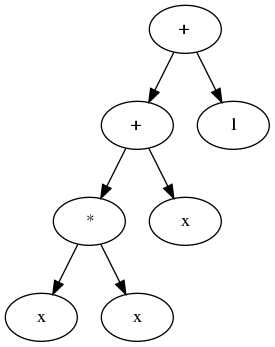
\includegraphics[width=70mm, height=70mm]{./Obrazky/formule_graph_2.png}
\caption{Strom výrazu}
\label{obr04:GrafFormule}
\end{figure}



\newpage
\section{Hluboké Q-učení}

% \subsection{Základní principy}
\subsection{Neuronová síť}
Než se dostaneme k hlubokému q-učení, budeme se nejprve muset seznámit s pojmy neuronová síť a q-učení. Začněme tedy s neurovnovými sítěmi.
Abychom si mohli říct, co neurovnové sítě jsou, musíme se nějdřív seznámit s její základní jednotku - perceptron.
\par
Perceptron je algoritmus, který má na vstupu několik hodnot $x_i$ a jeden výstup. S každou vstupní hodnotou je spojena jedna váha $w_i$.
Kromě váh vstupů obsahuje perceptron ještě tzv. práh. Perceptron spočítá vážený součet vstupů a porovná výsledek s prahem. Pokud je výsledek větší než práh, tak perceptron vrací hodnotu 1, jinak 0.
Můžeme zde ale využít triku pro zbavení se prahu. K práhu můžeme přistupovat jako k další váze s konstantním vstupem -1.
V takovém případě pak perceptron provádí porovnání váženého součtu vstupů s hodnotou 0. 
\newline
Matematicky zapsáno:
\[f(\sum_{i=0}^{n} w_if_i)\], kde $f$ vrací 1 pro $x>0$ a 0 jinak.

Trénování daného perceptronu probíhá pomocí předkládání dvojic vstupů a výstupů $(x,y)$ z trénovací množiny a upravování váh následujícím způsobem:
\newline
\[w_i = w_i + r(y-f(x_i)x_i\], kde $r$ je parametr učení.

Rozhodovací hranice perceptronu představuje nadrovinu ve vstupním prostoru. Lze ukázat, že trénování perceptronu zkonverguje, pokud jsou třídy v datech lineárně separabilní.

Většinou ale řešíme problémy, kde třídy v datech lineárně separabilní nejsou, v takových případech nám jeden perceptron nestačí a potřebujeme jich využít víc.
Spojením více perceptronů získáváme dopřednou neuronovou síť. Ta se skládá z vrstev perceptronů, kde vstupy perceptronů první jsou samotná data $x$ a vstupy perceptronů v dalších vrstávch jsou rovny výstupům perceptronů z vrstvy předchozí.

Pro trénování více vrstvých perceptronů se používá gradientní metoda. Z toho důvodů se využívají jiné funkce $f$, než ta zmíněná nahoře, ta má totiž gradient ve většíně případů roven 0.
Typickým příkladem používané funkce je sigmoid \[f(x) = \frac{1}{1+e^{-x}}\].

Následně musíme zvolit chybovou funkci $L(x,y|w)$ neuronové sítě. Zde se typicky využívá střední kvadratická chyba (ang. Mean squared error).
Chybová funkce se zderivuje podle vah v síti a následně se jednotlivé váhy upraví.
\newline
\[w_i = w_i + \alpha\frac{\partial L(x,y|w)}{\partial w_i}\]

\url{https://ocw.mit.edu/courses/health-sciences-and-technology/hst-947-medical-artificial-intelligence-spring-2005/lecture-notes/ch7_mach3.pdf}
\todo{strana 9 až 13}


\subsection{Zpětnovazební učení}
Podobně jako v předchozí sekci, i zde musíme nejprve zavést nové pojem a terminologii, než budeme moci říct, co je cílem zpětnovazebního učení.
Popišme si nejprve, co je to markovský rozhodovací prostor.
Markovský rozhodovací prostor popisuje prostředí a je definován čtveřicí $(S,A,P,R)$, kde $S$ je množina stavů, $A$ je množina všech akcí (případně $A_s$ představuje množinu akcí, které mohou být provedeny ve stavu $s$), 
$P: S \times A \times S \rightarrow [0,1]$ představuje přechodovou funkci, 
kde $P_a(s,s')$ vrací pravděpodobnost, že se aplikováním akce $a$ ve stavu $s$ dostaneme do stavu $s'$, 
a $R: S \times A \times S \rightarrow \mathbb{R}$ představuje funkci odměn $R_a(s,s')$, která vrací odměnu, kterou agent obdrží, pokud ve stavu $s$ provede akci $a$ a dostane se tak do stavu $s'$.
Přechodová funkce i funkce odměn musí navíc splňovat podmínku, že musí být jejich hodnoty nezávislé na předchozích stavech.

\url{https://ocw.mit.edu/courses/aeronautics-and-astronautics/16-410-principles-of-autonomy-and-decision-making-fall-2010/lecture-notes/MIT16_410F10_lec22.pdf}

Chování agenta v prostředí můžeme popsat pomocí strategie $\pi: S \times A \rightarrow [0,1]$, ta určuje pravděpodobnost, že se agent ve stavu $s$ rozhodne pro akci $a$.
Pro agenta v prostředí ještě definujme jeho celkovou odměnu jako \[\sum_{t=0}^{\infty} \gamma^tR_{a_t}(s_t,s_{t+1})\], kde $\gamma<1$ je diskontní faktor, díky kterému je suma konečná a $a_t$ je akce agenta vybraná v kroku t.
Cílem zpětnovazebního učení je nalézt optimální strategii $\pi^\star$, kde $a_t=\pi^\star(s_t)$, takovou, že její celková odměna je maximální.

Hodnotu stavu $s$ při použití strategie $\pi$ lze definovat jako 
\newline
\[V^{\pi}(s)=[\sum_{t=o}^{\infty} \gamma^tr_t|s_0=s]\], kde $r_t$ značí odměnu získanou v kroku t.
Podobně také můžeme definovat hodnotu $Q^{\pi}(s,a)$ akce $a$ provedené ve stavu $s$ při následování strategie $\pi$.
\[Q^\pi(s,a)=\sum_{s'}P_a(s,s')[R_a(s,s') + \gamma\sum_{a'} \pi(s',a')Q^\pi(s',a')]\]
Z Bellmanovy rovnice pro optimální strategie platí:
\[Q^*(s,a)=R_a(s,s') + \gamma\max_{a'}Q_k(s',a')\]

Agent ke zlepšování své strategie může využívat přechodové funkce a funkce odměn. Často ale agent hodnoty jednotlivých stavů předem nezná a musí se je učit za běhu.
Zároveň musí volit mezi explorací tj. prohledávání prostoru a exploatací tj. využívání známého. Zde využijeme $\epsilon$-hladového (ang. $\epsilon$-greedy) přístupu, kdy s pravděpodobností $\epsilon$ vybere náhodou akci a s pravděpodobností $1-\epsilon$ vybere nejlepší známou akci.

Nyní se už dostáváme ke Q-učení. $Q$ je reprezentována jako matice zpočátku inicializovaná samými nulami. Agent následně ve stavu $s_t$ vybírá například $\epsilon$-hladovým přístupem akci $a_t$, získá od prostředí odměnu $r_t$ a přesune se do stavu $s'$.
Na základě těchto informací se provede aktualizace matice následovně:
\newline
\[Q(s_t,a_t) \leftarrow (1-\alpha)Q(s_t,a_t) + \alpha(r_t + \gamma(\max_a(Q(s_{t+1},a))))\]




\subsection{Hluboké Q-učení}
Po seznámí se základy neuronových sítí a zpětnovazebního učení můžeme přejít k hlubokému Q-učení.
Hluboké Q-učení následuje stejnou myšlenku jako obyčejné Q-učení, také chceme nalézt odměnu vybrané akce v současném stavu stavu.
Hlavním rozdílem oproti normálnímu Q-učení je způsob jak se Q hodnoty reprezentují. V normálním Q-učení jsou Q hodnoty uložené v matici, ta může být v případě velkých prostorů příliš obrovská a Q-učení pak může probíhat velmi pomalu, nebo dokonce vůbec.
V Hlubokém Q-učení bude Q reprezentováno pomocí neuronové sítě.

Trénování se provádí pomocí porovnání rozdílu aktuální odměny $R_a(s,s')$ prostředí od odměny spočítané pomocí Bellmanovy rovnice z Q.
Cílem je tedy minimalizovat rozdíl mezi \[Q(s,a) \hspace{5mm}\text{a}\hspace{5mm}  R_a(s,s') + \gamma\max_{a'}Q_{\theta}(s',a')\], kde $Q_{\theta}$ jsou parametry neurovnové sítě reprezentující matici Q.
Chybovou funkcí pro trénování neuronové sítě pak může být střední čtvercová chyba tohoto rozdílu.



\subsection{Využití}
V praxi bylo hluboké Q-učení použito například pro naučení se hraní atari her. 
\url{https://www.cs.toronto.edu/~vmnih/docs/dqn.pdf}

Namísto ručně zpracovaných informacích o stavu hry zde byly jako vstupy využity přímo vizuální výstupy hry.
Q-síť je proto reprezentována konvoluční neuronovou sítí, která na vstupu bere vektor pixelů obrázku hry a na výstupu vrací odhad budoucích odměn pro každou z možných akcí.
Modelu nebylo řečeno nic o principu fungování hry. Model se učil pouze na základě vizuálního výstupu, odměn, které dostával od prostředí, konečných stavů a množiny možných akcí, tedy stejným přístupem, jak by ke hře přistupoval člověk.

Stejná neuronová síť byla použitá na sedmi různých atari hrách. Na šesti z nich překonala všechny stávající přístupy, které využívaly algoritmy zpětnovazebního učení a na třech z nich překonala výsledky nejlepších lidských hráčů.


